\documentclass[11pt,spanish] {article}
\def\spanishoptions{mexico}
\usepackage{mathptmx}
\usepackage{mwe,tikz}
\usepackage[percent]{overpic}
\usepackage[margin=0.5in]{geometry}
%~ \usepackage[spanish,es-noshorthands,es-ucroman]{babel}
\usepackage[spanish]{babel}
\usepackage{csvsimple}
\selectlanguage{spanish}
\usepackage[utf8]{inputenc}
%~ \usepackage{fancyhdr}
\usepackage[cm]{fullpage}
\usepackage{tabu}
\usepackage{hyperref}
%~ \pagestyle{fancy}
\usepackage[section]{placeins}
\usepackage{titlesec}
\usepackage{multirow}
\usepackage{graphicx}
\usepackage{makecell}
\usepackage{floatrow}
\usepackage{caption}
\usepackage{xcolor,colortbl}
%~ \usepackage{titling}
%~ \setlength{\droptitle}{-3cm}
\makeatletter
\def\input@path{{./public/latex/}}
%or: \def\input@path{{/path/to/folder/}{/path/to/other/folder/}}
\makeatother
\DeclareRobustCommand{\fecha}{02/ene/2021
}
\DeclareRobustCommand{\climatrimestre}{enero-febrero-marzo
}
\DeclareRobustCommand{\climaproximaactualizacion}{29/ene/2021
}
\DeclareRobustCommand{\situacionmeteorologica}{El Servicio Meteorológico Nacional mantiene diariamente la información
referente a la perspectiva meteorológica regional, con especial énfasis
en la parte de la cuenca sobre territorio argentino. Para los próximos
días se espera que prevalezcan condiciones de inestabilidad sobre la
mitad norte del Litoral. Se interpreta que el escenario abarcaría el
este de Paraguay la cuenca de aporte directo al embalse de Itaipú, las
cuenca baja del río Iguazú y la cuenca alta del río Uruguay. No se
espera que los eventos sean significativos.
}
\DeclareRobustCommand{\synoptext}{Se destaca pocos eventos de importancia y sobre áreas de respuesta
retardada. Las lluvias registradas en la última semana no alcanzan
magnitud como para alterar las tendencias hidrométricas en la región.
}
\DeclareRobustCommand{\situacionhidrologica}{\begin{itemize}
\tightlist
\item
  \textbf{Río Iguazú}:

  Sobre la cuenca baja se concentraron mayormente las lluvias, sin
  eventos importantes. Los acumulados variaron entre 20 mm y 50 mm. No
  es una mejora significativa, en momentos en que se redujo fuertemente
  el aporte de los afluentes a los embalses emplazados sobre el tramo
  medio del río. La regulación que realizan éstos determinó un caudal
  promedio semanal en Cataratas de 650 m3/s (sin cambios). No se espera
  una recuperación franca. Aún se mantiene a distancia de los bajísimos
  caudales registrados durante el pasado otoño. No se espera un franco
  retorno a valores normales en las próximas semanas. El promedio
  mensual en enero sería de 630 m3/s (60\% por debajo del promedio
  mensual de los últimos 25 años).
\item
  \textbf{Río Paraná desde Itaipú}:

  La cuenca del afluente Paranaiba volvió a concentrar las mayores
  lluvias, con una media espacial de los acumulados del orden de 50 mm.
  Sobre el resto de la alta cuenca los acumulados son poco
  significativos. El aporte de la parte regulada de la cuenca continúa
  oscilando y esta semana mostró una tendencia levemente descendente.
  Promedió 5.500 m3/s (un 5\% menos). No se espera un cambio importante
  en la próxima semana. El aporte de la mitad sur de la alta cuenca, la
  parte no regulada, aumentó levemente a unos 1.520 m3/s de promedio
  semanal, en gran medida por el aporte de las lluvias directas sobre el
  embalse de Itaipú. Dado el pronóstico meteorológico, en la próxima
  semana podría sostenerse en los actuales valores. El caudal entrante
  al embalse de Itaipú promedió 7.000 m3/s (3\% menos). La descarga del
  embalse volvió a reducirse, promediando unos 6.450 m3/s (8\% menos).
  Seguirá acotado en la próxima semana. El embalse de Itaipú va
  recuperando gradualmente su nivel y se ubica hoy a 2,90 m por debajo
  de la cota operativa normal. Probablemente este sea el cuarto verano
  consecutivo sin crecida estacional desde la alta cuenca del río
  Paraná.
\item
  \textbf{Confluencia Paraná-Iguazú}:

  El sensor de Puerto Iguazú correspondiente a la Red Hidrológica
  Nacional registró oscilaciones intradiarias con una leve tendencia
  descendente. El promedio semanal fue de 7,28 m (descenso promedio
  semanal de 1,00 m) y oscilando entre 4,85 m y 9,70 m. No se
  registraban valores tan bajos desde fines de mayo pasado. No se espera
  repunte significativo. Los máximos diarios promediarían en enero 7,75
  m (unos 8,00 m por debajo del promedio mensual desde 1996). La
  situación será monitoreada permanentemente con el equipo de mediciones
  de campo de la Red Hidrológica Nacional. El caudal en el Punto
  Trifinio promedió 7.160 m3/s (un 10\% menos).
\item
  \textbf{Tramo misionero-paraguayo del Paraná}:

  Sin lluvias de importancia. Sin cambios en la situación de la cuenca
  de aporte al tramo. El caudal entrante en ruta sigue sin repuntar y
  promediando valores muy bajos, muy por debajo de los 1.000 m3/s. En
  función del pronóstico meteorológico mencionado, podría registrarse un
  leve incremento durante la próxima semana.
\item
  \textbf{Tramo correntino-paraguayo del Paraná}:

  Sin lluvias de importancia. El caudal entrante al embalse de Yacyretá
  registró un promedio de 7.660 m3/s (8\% menos). La descarga promedió
  7.990 m3/s (10\% menos). El nivel en Paso de la Patria registró otro
  leve descenso promedio y quedó oscilando próximo a los 1,40 m (0,12 m
  de descenso promedio semanal). No se espera una recuperación en el
  corto plazo. Continuará en la franja de aguas bajas. Se mantendrá en
  esta condición en las próximas semanas.
\item
  \textbf{Río Paraguay en Cuenca Superior}:

  Se registró un resto de actividad sobre el Pantanal, con acumulados
  que puntualmente alcanzaron unos 90 mm. Sobre las nacientes las
  lluvias redujeron sensiblemente sus montos. Este escenario cambiante
  semana a semana no permite una recuperación franca de los caudales.
  Los niveles en todos los cursos de la alta cuenca registran un muy
  leve ascenso, a distancia de la franja de evolución normal
  correspondiente a esta época del año. No se espera nuevos eventos
  significativos en la próxima semana. Seguirá siendo muy acotado el
  aporte desde esa región hacia el tramo compartido argentino-paraguayo
  del río.
\item
  \textbf{Río Paraguay en Cuenca Media}:

  No se recuperaron las lluvias. La curva de recuperación estacional
  sigue retrasada. En Bahía Negra, en la descarga del Pantanal, el nivel
  presenta una leve tendencia ascendente, sin un ascenso franco por
  ahora. Hoy registró 0,95 m (0,90 m por debajo del promedio de enero
  desde 1996 y 0,50 m por debajo del nivel en igual fecha de 2020). En
  Puerto Concepción se observa un nivel estable, que hoy registró 1,10 m
  (1,71 m por debajo del normal de enero y 1,37 m por debajo del nivel
  en igual fecha de 2020).
\item
  \textbf{Río Paraguay en Cuenca Inferior}:

  Escasos eventos de importancia en la semana. El caudal fluvial desde
  el tramo medio del río redujo marcadamente y actualmente es de unos
  1.700 m3/s, un 23\% menos que en el domingo pasado. En Puerto
  Pilcomayo se registra hoy 1,33 m, con una caída en la semana de 0,70
  m. Se ubica en 1,71 m por debajo del promedio mensual de enero de los
  últimos 25 años y 2,27 m por debajo del nivel registrado en esta época
  en 2020). En el Puerto de Formosa el nivel se mantiene en acotado
  descenso desde el 27/dic. Se espera un leve descenso adicional. Hoy
  registró 2,00 m (2,02 m por debajo del promedio mensual de enero desde
  1996 y 1,99 m por debajo del nivel de igual fecha de 2020). Continuará
  en la franja de aguas bajas.
\item
  \textbf{Confluencia Paraná-Paraguay}:

  Los niveles en el área de confluencia nuevamente registraron descensos
  del orden de 0,10 m en promedio semanal. Los promedios semanales
  fueron de 1,47 m en Corrientes y de 1,55 m en Barranqueras. La
  perspectiva meteorológica no permite esperar una rápida recuperación.
  En enero los promedios mensuales serían de 1,55 m (unos 2,40 m por
  debajo de lo normal).
\item
  \textbf{Río Paraná en territorio argentino}:

  Escasas lluvias, sin eventos de importancia. El caudal que ingresa al
  tramo quedó oscilando próximo a los 10.500 m3/s, aún en leve
  disminución. Es del orden de un 35\% inferior al caudal promedio de
  enero de los últimos 25 años. Continuará siendo muy inferior a la
  referencia estadística. Los descensos semanales fueron en promedio
  entre 0,10 m y 0,20 m. Se acentúa la condición de aguas bajas. En Goya
  el nivel promediaría en enero 1,60 m (2,36 m por debajo de lo normal).
  En Santa Fe el nivel descendió a razón de 0,03 m por día. Promediaría
  en enero 1,10 m (2,45 m por debajo del valor normal). En el próximo
  día martes 05/ene/2021 se actualizarán los pronósticos a 7 días y las
  tendencias a 14 días.
\item
  \textbf{Delta del Río Paraná}:

  Sin lluvias de importancia. El caudal entrante al Delta se redujo al
  orden de los 11.000 m3/s, tendencia que se atenuaría en la próxima
  semana. La tendencia fluvial descendente se vio atenuada por los
  efectos de la crecida en el estuario durante el día viernes 01/ene.
  Resultaron entonces leves diferencias en términos de niveles promedio
  semanales. Se espera la persistencia del estiaje durante todo el
  verano. Los apartamientos actuales con respecto a los niveles medios
  habituales de esta época del año son de -2,25 m en Diamante y -1,64 m
  en Ramallo. En Victoria el nivel comenzó un gradual descenso. Se
  espere que mantenga la tendencia en la próxima semana. En Rosario el
  nivel promediaría en enero 0,75 m (2,49 m por debajo del nivel
  promedio desde 1996). No se espera una recuperación hacia niveles
  normales durante los tres próximos meses. En Villa Paranacito la
  crecida del estuario permitió una fugaz recuperación, retornando
  rápidamente a valores próximos a 1,00 m. Seguirá muy dependiente de
  las oscilaciones en el estuario. En referencia al Delta del Río
  Paraná, se recomienda visitar la página:
  https://www.ina.gob.ar/delta/index.php?seccion=1
\item
  \textbf{Río Gualeguay}:

  Prácticamente sin lluvias. Se observa niveles encauzados y sin
  tendencia definida. Gualeguay bajo: acusó brevemente el efecto de la
  crecida del estuario. La perspectiva para el trimestre al 31/mar/2021
  indica la continuidad del escenario de escasez sobre toda la
  Provincia. El monitoreo se realiza en conjunto con la Dirección
  General de Hidráulica de Entre Ríos. El último informe fue emitido el
  miércoles 23/dic y se presenta en la página web. El próximo informe
  sería elaborado el miércoles 06/ene/2021, con atención al monitoreo de
  variables hidrológicas regionales.
\item
  \textbf{Río Uruguay en su Alta Cuenca}:

  Sin eventos de importancia. Los embalses emplazados sobre el tramo
  superior del río continúan con niveles inferiores a los normales.
  Presentan entonces una importante capacidad de atenuación de los
  excedentes de futuras lluvias. El caudal de aporte al tramo compartido
  con Brasil se redujo fuertemente a menos de la mitad, promediando unos
  650 m3/s. El pronóstico meteorológico indica baja probabilidad de un
  repunte importante los próximos días.
\item
  \textbf{Cuenca Media del Río Uruguay}:

  Otra semana con escasas lluvias. El aporte de los afluentes es del
  orden de los 500 m3/s. No se espera un aumento significativo en la
  próxima semana. Predominó una tendencia descendente. Los niveles se
  mantienen próximos al límite de aguas bajas. En Paso de los Libres el
  caudal se mantuvo sin tendencia definido, promediando 1.350 m3/s. La
  tendencia climática indica lluvias de normales a inferiores a las
  normales sobre la cuenca media en el trimestre al 31/mar/2021. Se
  mantendrá la atención en los eventos de corto plazo.
\item
  \textbf{Cuenca Baja del Río Uruguay}:

  Escasas lluvias. El aporte total al embalse de Salto Grande promedió
  1.640 m3/s (casi sin cambios). El nivel de embalse siguió oscilando
  próximo a los 34,00 m. El tramo inferior presenta niveles próximos a
  la franja de aguas bajas, con dependencia de la evolución en el
  estuario. En Concepción del Uruguay el nivel promediaría en enero 1,10
  m (1,01 m por debajo del valor normal).
\item
  \textbf{Salado Santafesino}:

  Otra semana con escasas lluvias. Se observan niveles muy bajos en el
  tramo inferior. La Dirección General de Servicios Técnicos
  Específicos, dependiente del Ministerio de Infraestructura, Servicios
  Públicos y Hábitat de la Provincia se encuentra a cargo del monitoreo,
  manteniendo información sobre la evolución fluvial. No se espera un
  cambio sostenido y estable en las próximas semanas.
\item
  \textbf{Cuencas Bonaerenses}:

  Sin eventos significativos. No se espera una mejora sensible en la
  próxima semana. La perspectiva climática actualizada, válida para la
  Provincia y toda la llanura pampeana, con horizonte el 31/mar/2021
  próximo, mantiene la expectativa de lluvias inferiores a las normales.
\end{itemize}
}
\DeclareRobustCommand{\comentariofinal}{
}
\providecommand{\tightlist}{%
  \setlength{\itemsep}{0pt}\setlength{\parskip}{0pt}}
%~ \headheight 0pt
\setlength{\footskip}{10pt}
%~ \headsep 1pt 
\titlespacing*{\section}{0pt}{0ex}{0ex}
\graphicspath{{/home/alerta5/44-NODEJS_APIS/informe_complementario/public/latex/}}
\usepackage{tabularx}
\begin{document}
\captionsetup{labelformat=empty}
%~ \paragraph*{}
\begingroup
\begin{center}
\renewcommand{\arraystretch}{0.8}
\begin{tabularx}{\textwidth}{|c|>{\centering\arraybackslash}X|c|}
	\hline
	\multirow{5}{*}{
\includegraphics[height=1.7cm]{escudo_argentina.png}} & \textbf{\small{Ministerio de Obras Públicas}} & \multirow{5}{*}{
\includegraphics[width=2.6cm,height=1.3cm]{logo_ina_crop.png}}  \\
	& \textbf{\small{Secretaría de Infraestructura y Política Hídrica}} & \\
	& \textbf{\small{Subsecretaría de Obras Hidráulicas}} & \\
	& \textbf{\small{Instituto Nacional del Agua}} & \\ 
	& \textbf{\scriptsize{2021 - Año de Homenaje al Premio Nobel de Medicina Dr. César Milstein}} & \\ 
	\hline
	   \makecell{\textbf{Informe} \\ \textbf{complementario}} &  \makecell{\textbf{Situación meteorológica e hidrológica} \\ \textbf{Cuenca del Plata}} &  \fecha \\
	\hline
\end{tabularx}
\end{center}
\endgroup
%~ \paragraph*{}
%~ \vspace{1cm}
\begin{tabularx}{\textwidth}{|X|c|}
	\hline
	\multicolumn{2}{|c|}{\cellcolor{blue!25}Escenario Climático} \\
	\multicolumn{2}{|c|}{\cellcolor{blue!25}\climatrimestre} \\
	\hline
	\cellcolor{gray!25}\makecell{Próxima actualización : \\ Reunión mensual de análisis de las perspectivas climáticas en SMN} & \cellcolor{gray!25}\climaproximaactualizacion \\
	\hline
		\multicolumn{2}{|c|}{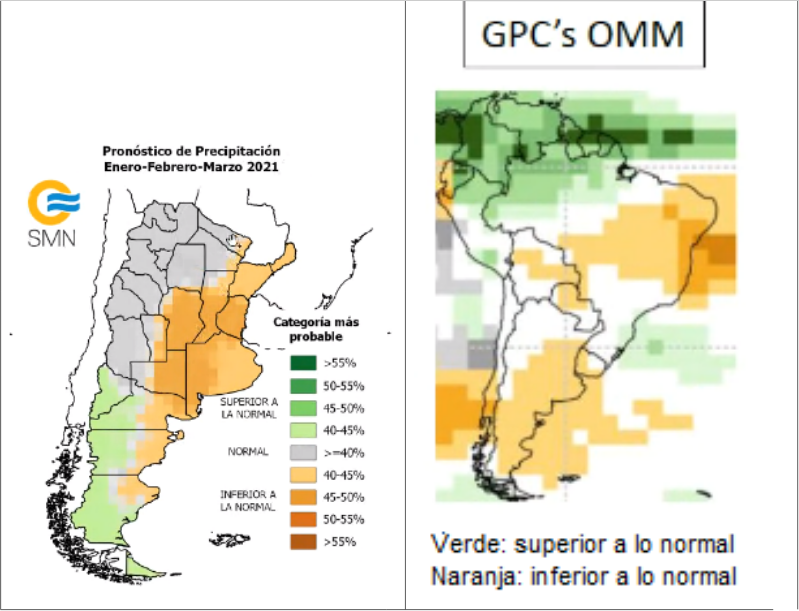
\includegraphics[height=10cm]{tendencia_climatica_file.png}} \\
		%~ 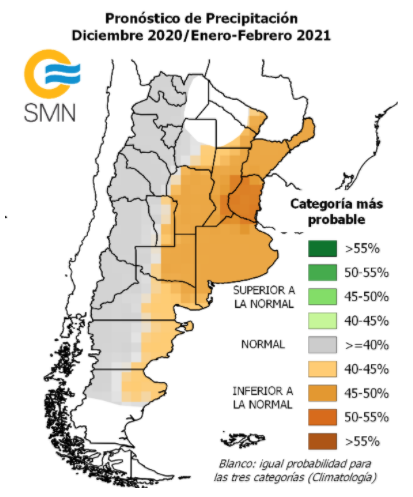
\includegraphics[width=9.3cm]{smn_map_file.png} & 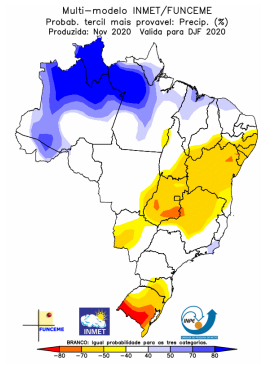
\includegraphics[width=9cm]{cptec_map_file.png} \\
	\hline
\end{tabularx}

\begin{figure}[H]
%~ \begin{tabular}{|c|p{8cm}|}
	%~ \hline
	\floatbox[{\capbeside\thisfloatsetup{capbesideposition={right,center},capbesidewidth=6cm}}]{figure}[\FBwidth]
	{\caption{\textbf{Precipitación acumulada semanal}\\\hspace{\textwidth}\\\hspace{\textwidth}\textbf{\synoptext}}\label{synopmap}}
	{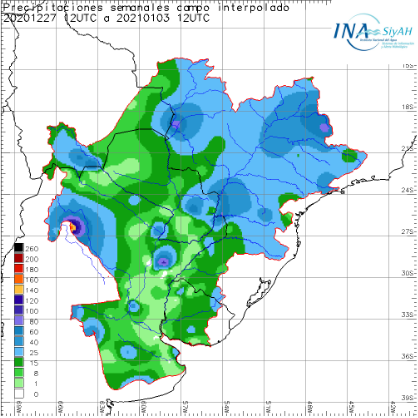
\includegraphics[height=8cm]{synop_semanal_file.png}}
		%~ 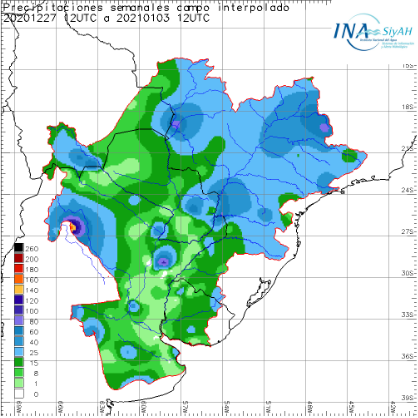
\includegraphics[width=10cm]{synop_semanal_file.png} & \textbf{Precipitación acumulada semanal} \textbf{\synoptext} \\  
	%~ \raisebox{9\normalbaselineskip}[0pt][0pt]
	%~ \hline
%~ \end{tabular}
\end{figure}
\situacionmeteorologica
\subsection*{Situación Hidrológica}
%~ \begin{itemize}
	\situacionhidrologica
	%~ \begin{itemize}
\tightlist
\item
  \textbf{Río Iguazú}:

  Sobre la cuenca baja se concentraron mayormente las lluvias, sin
  eventos importantes. Los acumulados variaron entre 20 mm y 50 mm. No
  es una mejora significativa, en momentos en que se redujo fuertemente
  el aporte de los afluentes a los embalses emplazados sobre el tramo
  medio del río. La regulación que realizan éstos determinó un caudal
  promedio semanal en Cataratas de 650 m3/s (sin cambios). No se espera
  una recuperación franca. Aún se mantiene a distancia de los bajísimos
  caudales registrados durante el pasado otoño. No se espera un franco
  retorno a valores normales en las próximas semanas. El promedio
  mensual en enero sería de 630 m3/s (60\% por debajo del promedio
  mensual de los últimos 25 años).
\item
  \textbf{Río Paraná desde Itaipú}:

  La cuenca del afluente Paranaiba volvió a concentrar las mayores
  lluvias, con una media espacial de los acumulados del orden de 50 mm.
  Sobre el resto de la alta cuenca los acumulados son poco
  significativos. El aporte de la parte regulada de la cuenca continúa
  oscilando y esta semana mostró una tendencia levemente descendente.
  Promedió 5.500 m3/s (un 5\% menos). No se espera un cambio importante
  en la próxima semana. El aporte de la mitad sur de la alta cuenca, la
  parte no regulada, aumentó levemente a unos 1.520 m3/s de promedio
  semanal, en gran medida por el aporte de las lluvias directas sobre el
  embalse de Itaipú. Dado el pronóstico meteorológico, en la próxima
  semana podría sostenerse en los actuales valores. El caudal entrante
  al embalse de Itaipú promedió 7.000 m3/s (3\% menos). La descarga del
  embalse volvió a reducirse, promediando unos 6.450 m3/s (8\% menos).
  Seguirá acotado en la próxima semana. El embalse de Itaipú va
  recuperando gradualmente su nivel y se ubica hoy a 2,90 m por debajo
  de la cota operativa normal. Probablemente este sea el cuarto verano
  consecutivo sin crecida estacional desde la alta cuenca del río
  Paraná.
\item
  \textbf{Confluencia Paraná-Iguazú}:

  El sensor de Puerto Iguazú correspondiente a la Red Hidrológica
  Nacional registró oscilaciones intradiarias con una leve tendencia
  descendente. El promedio semanal fue de 7,28 m (descenso promedio
  semanal de 1,00 m) y oscilando entre 4,85 m y 9,70 m. No se
  registraban valores tan bajos desde fines de mayo pasado. No se espera
  repunte significativo. Los máximos diarios promediarían en enero 7,75
  m (unos 8,00 m por debajo del promedio mensual desde 1996). La
  situación será monitoreada permanentemente con el equipo de mediciones
  de campo de la Red Hidrológica Nacional. El caudal en el Punto
  Trifinio promedió 7.160 m3/s (un 10\% menos).
\item
  \textbf{Tramo misionero-paraguayo del Paraná}:

  Sin lluvias de importancia. Sin cambios en la situación de la cuenca
  de aporte al tramo. El caudal entrante en ruta sigue sin repuntar y
  promediando valores muy bajos, muy por debajo de los 1.000 m3/s. En
  función del pronóstico meteorológico mencionado, podría registrarse un
  leve incremento durante la próxima semana.
\item
  \textbf{Tramo correntino-paraguayo del Paraná}:

  Sin lluvias de importancia. El caudal entrante al embalse de Yacyretá
  registró un promedio de 7.660 m3/s (8\% menos). La descarga promedió
  7.990 m3/s (10\% menos). El nivel en Paso de la Patria registró otro
  leve descenso promedio y quedó oscilando próximo a los 1,40 m (0,12 m
  de descenso promedio semanal). No se espera una recuperación en el
  corto plazo. Continuará en la franja de aguas bajas. Se mantendrá en
  esta condición en las próximas semanas.
\item
  \textbf{Río Paraguay en Cuenca Superior}:

  Se registró un resto de actividad sobre el Pantanal, con acumulados
  que puntualmente alcanzaron unos 90 mm. Sobre las nacientes las
  lluvias redujeron sensiblemente sus montos. Este escenario cambiante
  semana a semana no permite una recuperación franca de los caudales.
  Los niveles en todos los cursos de la alta cuenca registran un muy
  leve ascenso, a distancia de la franja de evolución normal
  correspondiente a esta época del año. No se espera nuevos eventos
  significativos en la próxima semana. Seguirá siendo muy acotado el
  aporte desde esa región hacia el tramo compartido argentino-paraguayo
  del río.
\item
  \textbf{Río Paraguay en Cuenca Media}:

  No se recuperaron las lluvias. La curva de recuperación estacional
  sigue retrasada. En Bahía Negra, en la descarga del Pantanal, el nivel
  presenta una leve tendencia ascendente, sin un ascenso franco por
  ahora. Hoy registró 0,95 m (0,90 m por debajo del promedio de enero
  desde 1996 y 0,50 m por debajo del nivel en igual fecha de 2020). En
  Puerto Concepción se observa un nivel estable, que hoy registró 1,10 m
  (1,71 m por debajo del normal de enero y 1,37 m por debajo del nivel
  en igual fecha de 2020).
\item
  \textbf{Río Paraguay en Cuenca Inferior}:

  Escasos eventos de importancia en la semana. El caudal fluvial desde
  el tramo medio del río redujo marcadamente y actualmente es de unos
  1.700 m3/s, un 23\% menos que en el domingo pasado. En Puerto
  Pilcomayo se registra hoy 1,33 m, con una caída en la semana de 0,70
  m. Se ubica en 1,71 m por debajo del promedio mensual de enero de los
  últimos 25 años y 2,27 m por debajo del nivel registrado en esta época
  en 2020). En el Puerto de Formosa el nivel se mantiene en acotado
  descenso desde el 27/dic. Se espera un leve descenso adicional. Hoy
  registró 2,00 m (2,02 m por debajo del promedio mensual de enero desde
  1996 y 1,99 m por debajo del nivel de igual fecha de 2020). Continuará
  en la franja de aguas bajas.
\item
  \textbf{Confluencia Paraná-Paraguay}:

  Los niveles en el área de confluencia nuevamente registraron descensos
  del orden de 0,10 m en promedio semanal. Los promedios semanales
  fueron de 1,47 m en Corrientes y de 1,55 m en Barranqueras. La
  perspectiva meteorológica no permite esperar una rápida recuperación.
  En enero los promedios mensuales serían de 1,55 m (unos 2,40 m por
  debajo de lo normal).
\item
  \textbf{Río Paraná en territorio argentino}:

  Escasas lluvias, sin eventos de importancia. El caudal que ingresa al
  tramo quedó oscilando próximo a los 10.500 m3/s, aún en leve
  disminución. Es del orden de un 35\% inferior al caudal promedio de
  enero de los últimos 25 años. Continuará siendo muy inferior a la
  referencia estadística. Los descensos semanales fueron en promedio
  entre 0,10 m y 0,20 m. Se acentúa la condición de aguas bajas. En Goya
  el nivel promediaría en enero 1,60 m (2,36 m por debajo de lo normal).
  En Santa Fe el nivel descendió a razón de 0,03 m por día. Promediaría
  en enero 1,10 m (2,45 m por debajo del valor normal). En el próximo
  día martes 05/ene/2021 se actualizarán los pronósticos a 7 días y las
  tendencias a 14 días.
\item
  \textbf{Delta del Río Paraná}:

  Sin lluvias de importancia. El caudal entrante al Delta se redujo al
  orden de los 11.000 m3/s, tendencia que se atenuaría en la próxima
  semana. La tendencia fluvial descendente se vio atenuada por los
  efectos de la crecida en el estuario durante el día viernes 01/ene.
  Resultaron entonces leves diferencias en términos de niveles promedio
  semanales. Se espera la persistencia del estiaje durante todo el
  verano. Los apartamientos actuales con respecto a los niveles medios
  habituales de esta época del año son de -2,25 m en Diamante y -1,64 m
  en Ramallo. En Victoria el nivel comenzó un gradual descenso. Se
  espere que mantenga la tendencia en la próxima semana. En Rosario el
  nivel promediaría en enero 0,75 m (2,49 m por debajo del nivel
  promedio desde 1996). No se espera una recuperación hacia niveles
  normales durante los tres próximos meses. En Villa Paranacito la
  crecida del estuario permitió una fugaz recuperación, retornando
  rápidamente a valores próximos a 1,00 m. Seguirá muy dependiente de
  las oscilaciones en el estuario. En referencia al Delta del Río
  Paraná, se recomienda visitar la página:
  https://www.ina.gob.ar/delta/index.php?seccion=1
\item
  \textbf{Río Gualeguay}:

  Prácticamente sin lluvias. Se observa niveles encauzados y sin
  tendencia definida. Gualeguay bajo: acusó brevemente el efecto de la
  crecida del estuario. La perspectiva para el trimestre al 31/mar/2021
  indica la continuidad del escenario de escasez sobre toda la
  Provincia. El monitoreo se realiza en conjunto con la Dirección
  General de Hidráulica de Entre Ríos. El último informe fue emitido el
  miércoles 23/dic y se presenta en la página web. El próximo informe
  sería elaborado el miércoles 06/ene/2021, con atención al monitoreo de
  variables hidrológicas regionales.
\item
  \textbf{Río Uruguay en su Alta Cuenca}:

  Sin eventos de importancia. Los embalses emplazados sobre el tramo
  superior del río continúan con niveles inferiores a los normales.
  Presentan entonces una importante capacidad de atenuación de los
  excedentes de futuras lluvias. El caudal de aporte al tramo compartido
  con Brasil se redujo fuertemente a menos de la mitad, promediando unos
  650 m3/s. El pronóstico meteorológico indica baja probabilidad de un
  repunte importante los próximos días.
\item
  \textbf{Cuenca Media del Río Uruguay}:

  Otra semana con escasas lluvias. El aporte de los afluentes es del
  orden de los 500 m3/s. No se espera un aumento significativo en la
  próxima semana. Predominó una tendencia descendente. Los niveles se
  mantienen próximos al límite de aguas bajas. En Paso de los Libres el
  caudal se mantuvo sin tendencia definido, promediando 1.350 m3/s. La
  tendencia climática indica lluvias de normales a inferiores a las
  normales sobre la cuenca media en el trimestre al 31/mar/2021. Se
  mantendrá la atención en los eventos de corto plazo.
\item
  \textbf{Cuenca Baja del Río Uruguay}:

  Escasas lluvias. El aporte total al embalse de Salto Grande promedió
  1.640 m3/s (casi sin cambios). El nivel de embalse siguió oscilando
  próximo a los 34,00 m. El tramo inferior presenta niveles próximos a
  la franja de aguas bajas, con dependencia de la evolución en el
  estuario. En Concepción del Uruguay el nivel promediaría en enero 1,10
  m (1,01 m por debajo del valor normal).
\item
  \textbf{Salado Santafesino}:

  Otra semana con escasas lluvias. Se observan niveles muy bajos en el
  tramo inferior. La Dirección General de Servicios Técnicos
  Específicos, dependiente del Ministerio de Infraestructura, Servicios
  Públicos y Hábitat de la Provincia se encuentra a cargo del monitoreo,
  manteniendo información sobre la evolución fluvial. No se espera un
  cambio sostenido y estable en las próximas semanas.
\item
  \textbf{Cuencas Bonaerenses}:

  Sin eventos significativos. No se espera una mejora sensible en la
  próxima semana. La perspectiva climática actualizada, válida para la
  Provincia y toda la llanura pampeana, con horizonte el 31/mar/2021
  próximo, mantiene la expectativa de lluvias inferiores a las normales.
\end{itemize}

%~ \end{itemize}

\center{\textbf{\underline{Se recomienda visitar la página web para observar los productos del monitoreo satelital}}} \\
\begin{tabular}{c}
\href{https://alerta.ina.gob.ar/pub/mapa}{https://alerta.ina.gob.ar/pub/mapa} (mapa) \\
\href{https://alerta.ina.gob.ar/pub/gui}{https://alerta.ina.gob.ar/pub/gui} (listado de servicios) \\
\href{https://alerta.ina.gob.ar/ina}{https://alerta.ina.gob.ar/ina} (repositorio de mapas, gráficas e informes) \\
\end{tabular}
\center{\comentariofinal}
\subsubsection{Referencias}
\begin{tabularx}{\textwidth}{|X|c|}
	\hline
	Prefectura Naval Argentina & Comisión Técnica Mixta de Salto Grande \\
	\hline
	Servicio Meteorológico Nacional & Comisión Regional del Bermejo \\
	\hline
	Entidad Binacional Yacyretá & Ministerio de Infraestructura y Transporte de la Provincia de Santa Fe \\
	\hline
	ONS (Brasil) & CPRM (Brasil) \\
	\hline
\end{tabularx}
\end{document}

